\begin{title}
  Глава 1
\end{title}

\begin{title}
  Теория кривых
\end{title}

\begin{title}
  Параграф 1
\end{title}

\begin{title}[\Large]
  Определение и способы задания кривых
\end{title}

\begin{define}[кривой]
  Непрерывной кривой называется непрерывное отображение
  $$
  \varphi: [a,b] \to R^3 ~~~ \varphi = \varphi (t), ~~~ t \in [a,b]
  $$
  $\varphi ([a,b]) \subseteq R$ - называется образом кривой

  $\vec \varphi (t) = ( x(t), y(t), z(t) )$ вектор

  $x = x(t); ~ y = y(t); ~ z = z(t)$ - называются координатами функции

  Параметрическое уравнение кривой $\varphi(t) = ( x(t), y(t), z(t) )$
  $$
  \left\{
  \begin{array}{c}
    x = x(t) \\
    y = y(t) \\
    z = z(t)
  \end{array}
  \right.
  $$
\end{define}

\begin{define}[гладкой кривой]
  $\vec \varphi = ( x(t), y(t), z(t) )$ называется гладкая если каждая координата
  является гладкой. Гладкая значит что существует производная любого порядка.
\end{define}

\begin{define}[касательного вектора к кривой]
  Касательный вектор кривой или вектор скорости называется
  $$
  \varphi' (t) = ( x'(t), y'(t), z'(t) ) ~~ \text{или} ~~
  \lim_{ t_{\Delta} \to 0 }
  \frac{ \vec \varphi (t + t_{\Delta}) - \vec \varphi (t) }{t_{\Delta}}
  $$

  Если кривая образует угол то точка этого угла $t_0$ называется собой и
  $\vec \varphi (t_0) = \vec 0$
\end{define}

\begin{define}[регулярной кривой]
  $\vec \varphi = \vec \varphi (t)$ называется регулярной если
  $\forall t ~~ \vec \varphi' (t) \not = \vec 0$
\end{define}

\begin{define}[инективности и неинективности]
  Инективно - значит нескольким точкам соответсвует одно значение.

  Неинективно - значит каждой точке соответсвует одно значение.
\end{define}

\begin{theorem}
  Пусть $\varphi : [a,b] \to R^3$ - гладкая кривая, $t_0 \in (a,b)$
  $\vec \varphi' (t_0) \not = 0$ тогда $\exists \varepsilon > 0$
  $\varphi : (t_0 - \varepsilon, t_0 + \varepsilon) \to R^3$ инективно.
\end{theorem}

\begin{define}[касательной прямой регулярной кривой]
  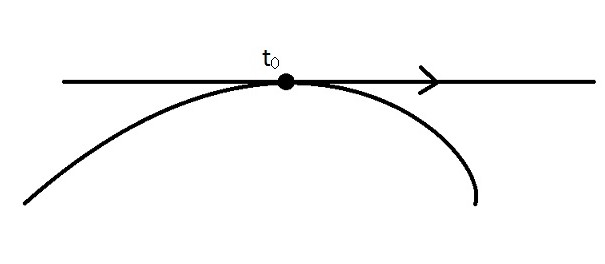
\includegraphics[width = 4.5cm]{tangent}

  $\varphi' (t_0) \not = \vec 0$ тогда касательная прямая
\end{define}

\begin{define}[касательной плоскости]
  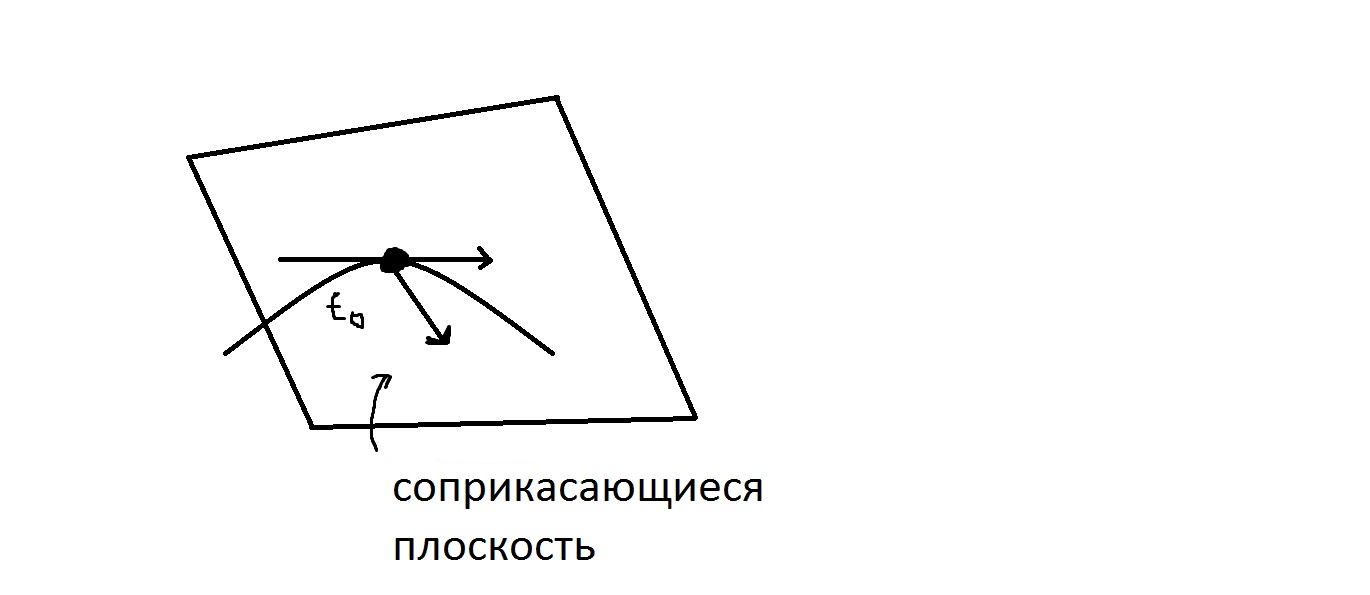
\includegraphics[width = 6cm]{beleg}

  Соприкасающиейся  л.н.з (некомпланарная) плоскость.
\end{define}

\begin{define}[бирегулярности]
  $t_0$ называется точкой биригулярности, если $\vec \varphi' (t_0) ~~~
  \vec \varphi''(t_0)$ - линейно независимы (неколинеарны).
\end{define}

\begin{define}[бирегулярности кривой]
  $\vec \varphi = \vec p(t)$ называется биригулярной если все ее точки являются
  точками билигулярности

  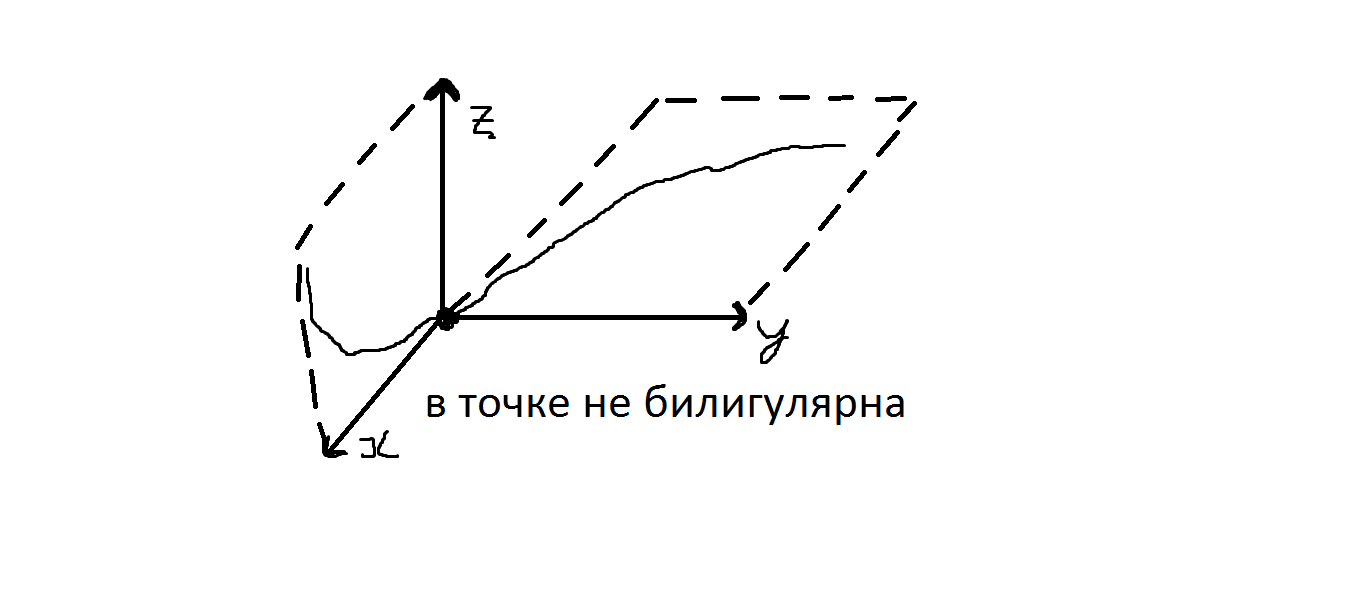
\includegraphics[width = 6cm]{notBeleg}
\end{define}

\begin{define}[диффеоморфизма]
  Диффеоморфизмом называется гладкое отображение при котором обратное
  отображение тоже гладкое.
\end{define}

Биективное отображение гладкое в обе стороны.

\begin{define}
  Пусть даны две кривые

  $\varphi_1 : [a,b] \to R^3$

  $\varphi_2 : [a,b] \to R^3$

  называются эквивалентными если существует диффeoморфизм
  $\varphi : [a,b] \to [\alpha, \beta]$ или $\varphi_2(\varphi(t)) =
  \varphi_1(t)$
\end{define}

Параметризация эквивалентных прямых называется эквивалентными если все кривые
разбиваются на классы эквивалентных кривых эти классы классы эквивалентности
кривых называются разными параметризациями кривых.

\begin{theorem}
  Расмотрим множество точек заданным соотношением $F(x, y) = 0$ - гладкая.
  Пусть $\exists (x_0, y_0) ~~~ F(x_0, y_0) = 0$
  $$
  \grad F(x_0, y_0) = \left( \frac{\partial F}{\partial x}(x_0, y_0);
  \frac{\partial F}{\partial y}(x_0, y_0) \right)
  $$
  тогда $\exists O(x_0, y_0)$ в которой множество точек удовлитворяет
  $F(x, y) = 0$ является образом регулярной кривой

  В этом случа мы будем говорить что это регулярная кривая задана неявно
  соотношением $F(x, y) = 0$.
\end{theorem}

\begin{theorem}[о неявных функциях]
  Пусть  даны гладкие функции
  $$
  \begin{array}{c}
    F_1 (x_1, x_2, \cdots, x_n, y_1, y_2, \cdots, y_m) \\
    \dots ~~~ \dots ~~~ \dots ~~~ \dots  ~~~ \dots ~~~ \dots \\
    F_m (x_1, x_2, \cdots, x_n, y_1, y_2, \cdots, y_m)
  \end{array}
  $$
  тогда если точка $(x_0, y_0)$ такова что
  $$
  \begin{array}{c}
    F_1(x_0, y_0) = 0 \\
    \ldots ~~~ \ldots \\
    F_m(x_0, y_0) = 0 \\
  \end{array} ~~~~~~
  \left|
  \begin{array}{ccc}
    \frac{\partial F_1}{\partial y_1} & \dots &
    \frac{\partial F_1}{\partial y_1} \\

    \dots & \dots & \dots \\

    \frac{\partial F_m}{\partial y_1} & \dots &
    \frac{\partial F_m}{\partial y_m} \\
  \end{array}
  \right|
  \not= 0
  $$
  то $\exists O(x_0, y_0)$ в которой точки улидотворяющие соотношением
  $$
  \left\{
  \begin{array}{c}
    F_1(x, y) = 0 \\
    \dots ~~~ \dots \\
    F_m(x, y) = 0
  \end{array}
  \right. ~~~ \text{задаются} ~~~
  \left\{
  \begin{array}{c}
    y_1 = f_1(x_1, x_2, \cdots, x_n) = 0 \\
    \dots ~~~ \dots ~~~ \dots ~~~ \dots \\
    y_n = f_m(x_1, x_2, \cdots, x_n) = 0
  \end{array}
  \right.
  $$
  для некоторых гладких функций $f_1, f_2, \cdots, f_m $
\end{theorem}

\begin{proof}
  По условию  точка $(x_0, y_0)$
  $$
  \grad F(x_0, y_0) = \left( \frac{\partial F}{\partial x}(x_0, y_0);
  \frac{\partial F}{\partial y}(x_0, y_0) \right) \not= 0
  $$
  Можем считать что $\frac{\partial F}{\partial y}(x_0, y_0) \not= 0$ по
  теореме о неявной функции $\exists (x, y) \in O(x_0, y_0) ~~~ F(x, y) = 0$
  задается соотношением $y = f(x)$
  тоисть состоит из точек вида $(x, f(x))$ следовательно это множество точек
  задается параметрически уравнением $\vec \varphi (t, f(t))$

  $\vec \varphi = (1, f'(x)) \not= 0$ следовательно кривая заданная этим
  уравнением регулярная.
\end{proof}

Покажем что для кривой неявно заданной соотношением $f(x, y) = 0$ вектор
градиента является нормалью (перпендикулярью касательной кривой) и направлен в
сторону выпуклости кривой.

По теореме наша кривая может быть задана параметрической кривой
$\vec \varphi = (x(t), y(t))$ тогда
$$
F(x(t), y(t)) = 0 ~~~
\frac{dF}{dt} = \frac{\partial F}{\partial x} \dots \frac{dx}{dt} +
\frac{\partial F}{\partial x} \dots \frac{dy}{dt} =
(\grad F, \vec \varphi') = 0 ~ \Rightarrow ~ \grad F \perp \varphi'
$$